\section{Implementation and Experiments}
\label{sec:exp}

In this section, we will show our details on our implementations and report the result as required from the 3 tasks.

\subsection{Implementation Details}
\label{subsec:implement}

This project is implemented in pure C++ using minimum version 17. The block size is determined based on the system settings and statistics of the running machine. Therefore, different machines may result in varying block sizes. For simplicity, we use a block size of 4096, which is the default setting on most machines, throughout the rest of the paper unless otherwise specified.

\subsection{Task 1}
\label{subsec:task1}

\begin{table}[ht]
    \begin{minipage}{.55\textwidth}
        \renewcommand{\arraystretch}{1.2}
        \resizebox{0.95\textwidth}{!}{
        \begin{tabular}{@{}lll@{}}
            \toprule
            \textbf{Column Name} & \textbf{Data Type} & \textbf{Row Size} (Bytes)\\
            \midrule
            \texttt{GAME\_DATE\_EST}       & \texttt{DATE}             & 10   \\
            \texttt{TEAM\_ID\_home}        & \texttt{VARCHAR(10)}      & 10  \\
            \texttt{PTS\_home}             & \texttt{INT}              &  4  \\
            \texttt{FG\_PCT\_home}         & \texttt{FLOAT32}          &  4  \\
            \texttt{FT\_PCT\_home}         & \texttt{FLOAT32}          &  4  \\
            \texttt{FG3\_PCT\_home}        & \texttt{FLOAT32}          &  4  \\
            \texttt{AST\_home}             & \texttt{INT}              &  4  \\
            \texttt{REB\_home}             & \texttt{INT}              &  4  \\
            \texttt{HOME\_TEAM\_WINS}      & \texttt{BOOLEAN}          &  1  \\
            \midrule
            \textbf{Total}        &                  & 45 \\
            \bottomrule
        \end{tabular}
        }
        \vspace{2mm}
        \caption{Fields statistics inside a record}
        \label{tab:field-stats}
    \end{minipage}
    \hfill
    \begin{minipage}{.4\textwidth}
        \centering
        \renewcommand{\arraystretch}{1.2}
        \begin{tabular}{@{}lll@{}}
        \toprule
        File                   & Num. of lines   & 26651 \\
        \midrule
        \multirow{2}{*}{Record}& Num. of records & 26651 \\
                               & Size (Bytes)    & 45    \\
        \midrule
        \multirow{2}{*}{Block} & Num. of blocks  & 293   \\
                               & Size (Bytes)    & 4096  \\
        \bottomrule
        \end{tabular}
        \vspace{5mm}
        \caption{The size of a record; The number of
records; The number of records stored in a block; The number of blocks
for storing the data}
    \end{minipage}
\end{table}

\vspace{-2mm}

\paragraph{Record} In our database system, and in the provided \textit{games.txt} file, a record consists of an array of 45 bytes. A detailed explanation of how we chose the data types and corresponding row sizes for each field is provided in \Cref{tab:field-stats}. Examples of the converted byte arrays for different data types can be found in \Cref{fig:storage-component}. Since there are 26651 lines in the txt file, there will be 26651 records in the database.

\paragraph{Block} Our block size is set to the default value of 4096 bytes. Therefore, each block can store $\left\lfloor \frac{4096}{45} \right\rfloor = 91$ records. To store all the records in our database, we will need $\left\lceil\frac{26651}{91}\right\rceil = 293$ blocks.

\paragraph{Database File} A database file in our system is a binary file named with the extension \textit{.db}. It contains multiple blocks used to store the database’s data.


\subsection{Task 2}
\label{subsec:task-2}

\paragraph{Degree $t$} In our \bplustree structure, degree (t) is the minimum number of subtrees of an internal node. In our \bplustree, the degree is $102$.

\begin{table}[h]
    \hfill
    \begin{minipage}{.99\textwidth}
        \centering
        \renewcommand{\arraystretch}{1.2}
        \begin{tabular}{@{}lll@{}}
        \toprule
        Statistic                   & Value       \\
        \midrule
        \multirow{1}{*}{Parameter \textit{n}}& 203 \\

        \midrule
        \multirow{1}{*}{Total number of nodes} & 266  \\

        \midrule
        \multirow{1}{*}{Number of levels} & 3 \\

        \midrule
        \multirow{1}{*}{Content of root node} & 3 keys from the file \\

        \bottomrule
        \end{tabular}
        \vspace{5mm}
        \caption{the parameter $n$ of the \bplustree; the
number of nodes of the \bplustree; the number of levels of the \bplustree; the content of the root node}
    \end{minipage}
\end{table}

\paragraph{Parameter $n$} The parameter $n$ is restricted to be an odd integer, which refers to the maximum number of keys that can be stored in a node; and it is equal to two times degree minus $1$, which is $2\times 102-1=203$.

\paragraph{Number of Nodes} There are $26,651$ records. Since each leaf node must store at least $102$ keys, the minimum number of leaf nodes is $\left\lceil\frac{26651}{102}\right\rceil = 262$, So there will be $262$ leaf nodes in this case. Each internal node can have at least $102$ pointers (since internal nodes must have at least
$t=102$ children). Therefore, the number of internal nodes at the first level is $\left\lceil \frac{262}{102} \right\rceil = 3$. Since there are only $3$ internal nodes in the first level, the second level will contain $1$ root node (because the root can store at least $101$ keys and have up to $102$ children). Therefore, totally there are $262 + 3 + 1 = 266$ nodes.

\paragraph{Number of levels in the \bplustree} For leaf level there are 262 leaf nodes; at first internal level there are 3 internal nodes; at root Level there are 1 root node. Therefore, the \bplustree has \textbf{3 levels}.

\paragraph{Content of the root node (only the keys)} The root node will contain the first keys from each of its 3 children (the internal nodes). Since there are only 3 internal nodes, the root will contain 3 keys that guide the search process to the appropriate internal node.

\subsection{Task 3}
\label{subsec:task-3}

\begin{figure*}[h]
    \centering
    \begin{subfigure}[t]{0.45\textwidth}
        \centering
        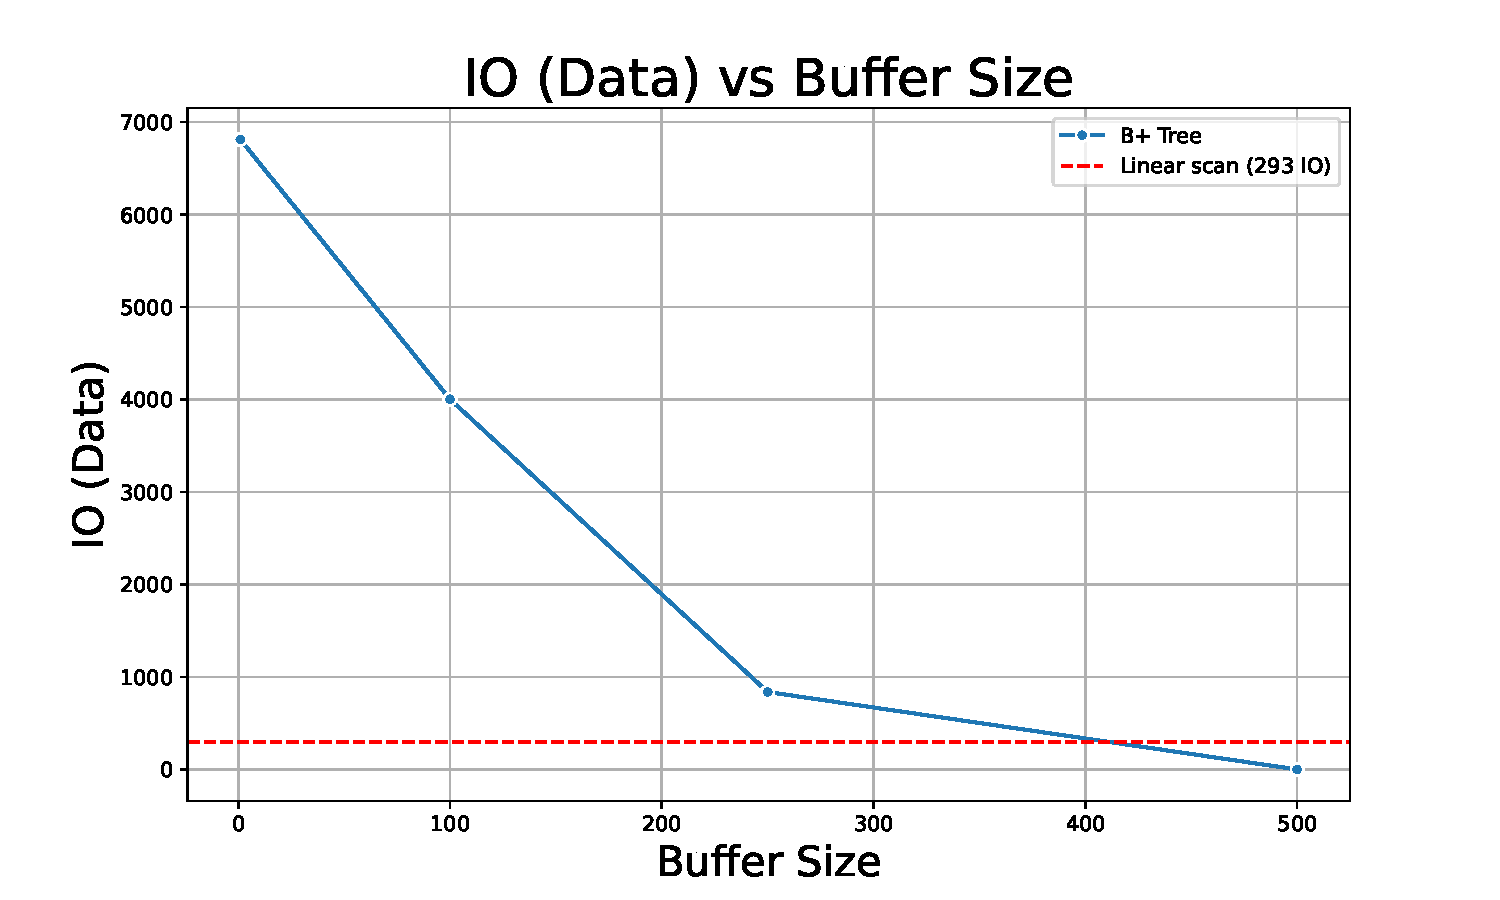
\includegraphics[width=0.95\linewidth]{figures/block_io_vs_buffer_size.pdf}
        \caption{Comparison between different buffer size and data block access for \bplustree}
    \end{subfigure}%
    ~
    \begin{subfigure}[t]{0.45\textwidth}
        \centering
        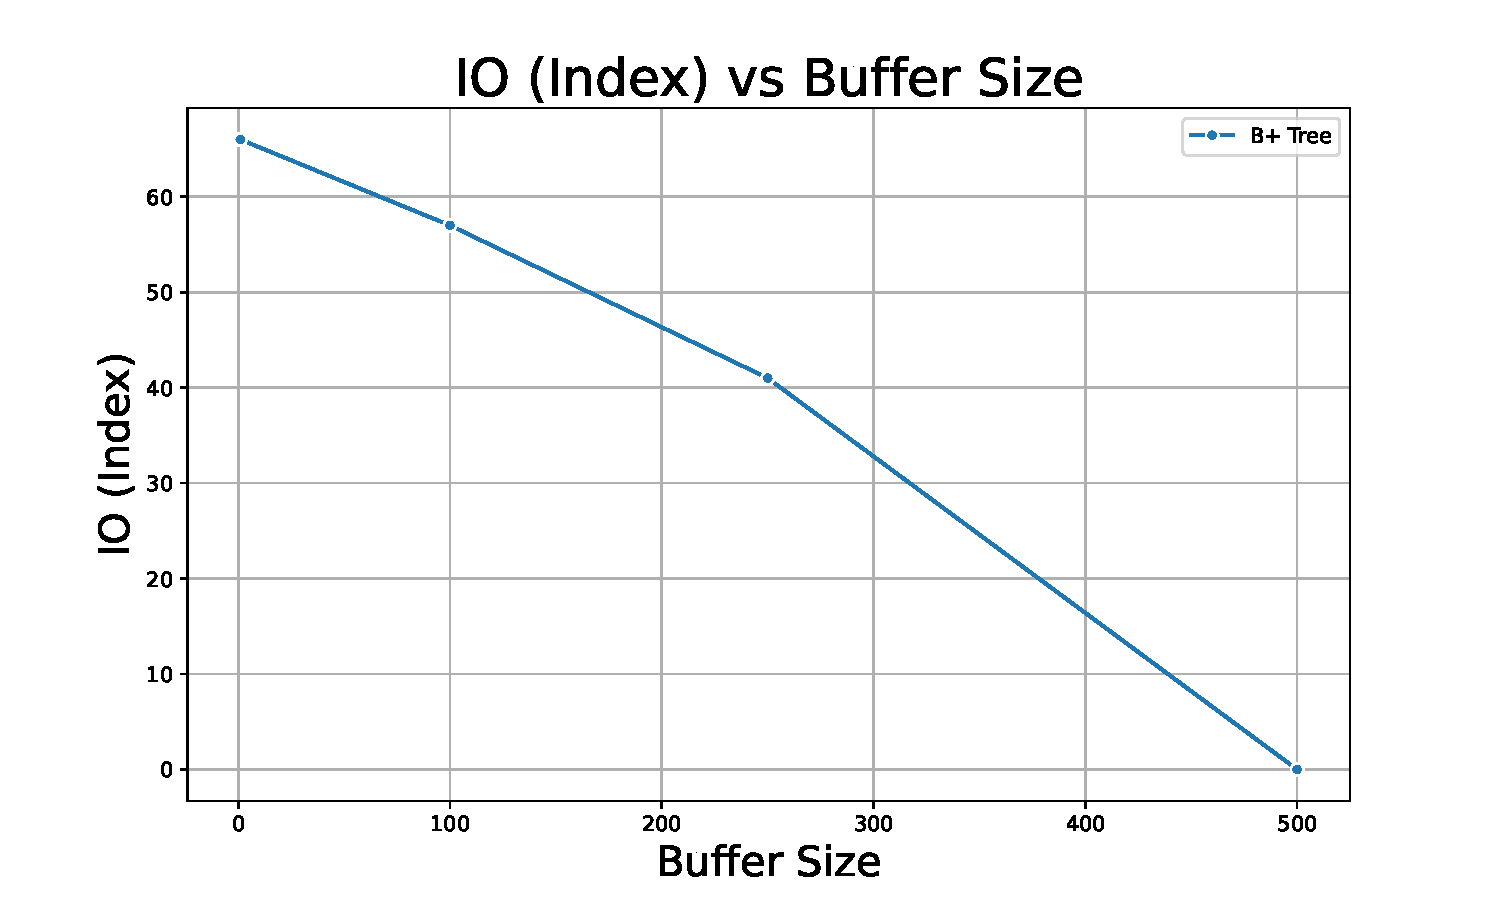
\includegraphics[width=0.95\linewidth]{figures/index_io_vs_buffer_size.pdf}
        \caption{Comparison between different buffer size and index block access for \bplustree}
    \end{subfigure}
    \vspace{3mm}

    \begin{subfigure}[t]{0.55\textwidth}
        \centering
        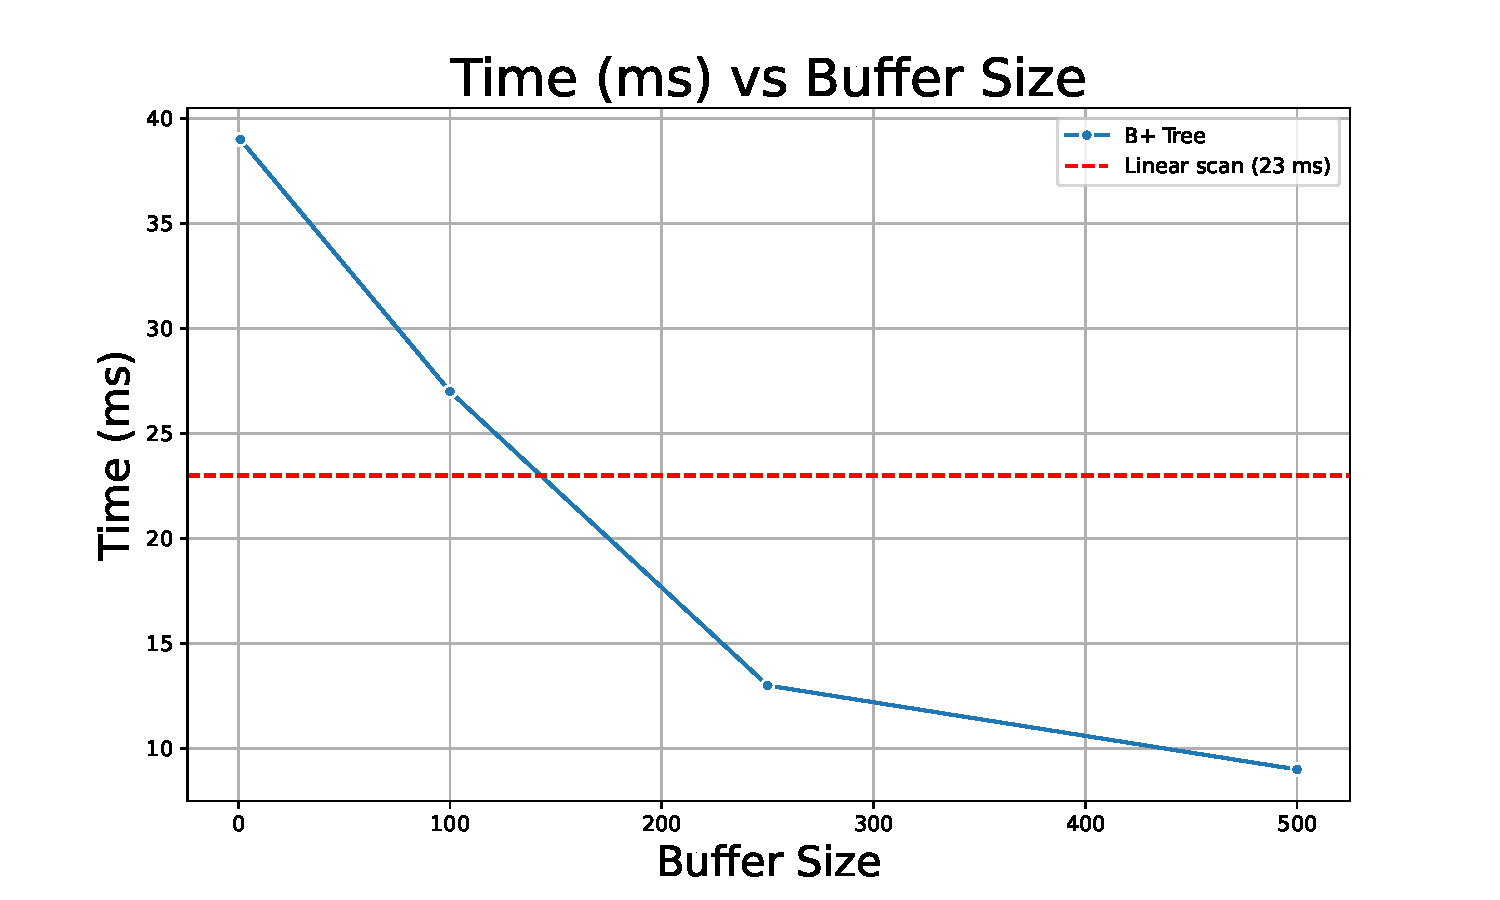
\includegraphics[width=0.95\linewidth]{figures/time_vs_buffer_size.pdf}
        \caption{Comparison between different buffer size and runtime for \bplustree and linear scan}
        \label{subfig:time-vs-buffer}
    \end{subfigure}
    \caption{Exploring different buffer size}
\end{figure*}


\begin{table}[h]
\begin{minipage}{0.55\textwidth}
\resizebox{0.95\textwidth}{!}{
\begin{tabular}{@{}l|ll|ll}
\toprule
Buffer Size & \textsc{Time} ($\mu s$) & \textsc{Time} ($ms$) & \textsc{IO} (Index Block) & \textsc{IO} (Data Block)  \\
\midrule
1            & 39774              & 39       & 66   &   6812 \\
% 10           & 39810              & 39       & 87   &   6265 \\
% 50           & 34176              & 34       & 114  &   5100 \\
100          & 27891              & 27       & 57   &   4003 \\
250          & 13469              & 13       & 41   &   838  \\
500          & 9351               & 9        & 0    &   0    \\
\bottomrule
\end{tabular}
}
\vspace{2mm}
\caption{The number of IO and time for different buffer sizes using B+ tree. Our indexes are built in a non-clustered order and thus may access a data block multiple times and getting the result}
\label{tab:io-tab}
\end{minipage}
\hfill
\begin{minipage}{0.4\textwidth}

\resizebox{0.95\textwidth}{!}{
\centering
\renewcommand{\arraystretch}{1.2}
\begin{tabular}{l|ccc}
\toprule
Method           & IO (Index) & IO (Data) & Time (ms) \\
\midrule
Linear Scan      & 0          & 293       & 22        \\
\bplustree          & 66         & 6812      & 39        \\
\bplustree w. cache & 41         & 838       & 13        \\
\bottomrule
\end{tabular}
}
\vspace{2mm}
\caption{Comparison with different methods: Linear Scan, B+ tree, B+ tree with cache. The cache of the B+ tree is set to be 250 pages.}
\label{tab:comparison}

\end{minipage}

\end{table}

We will now present the statistics required for Task 3. The results were obtained by running the system with different buffer sizes, and the outcomes are summarized in \Cref{tab:io-tab,tab:comparison}.

\paragraph{Index Node Access} Without using a buffer\footnote{The minimum buffer size for our program is 1 since we always update our buffer after reading one block. However, in this scenario, this buffer would not have any effect. Thus, we consider the case when buffer size is 1 as no buffer.}, the number of I/O operations for accessing index blocks is 66, which is approximately equal to $\lfloor \frac{6902}{102} \rfloor = 67$, where 6902 is the number of records that satisfy the query conditions. As the buffer size increases, the number of I/O operations for accessing the index decreases gradually, as portions of the index are stored in the buffer during the building phase.

\paragraph{Data Block Access} Since we use a dense non-clustered index, many data blocks are accessed multiple times because the records are not stored sequentially, the number of I/O operations for accessing data blocks is 6812, which is much greater than using linear scan. The high I/O in data block access results in the runtime of the B+ tree being longer than that of the range query. This issue can be mitigated by increasing the buffer size, as the linear scan cannot fully utilize the buffer, and the B+ tree will have a shorter runtime with an increased buffer size.

\paragraph{Average of ``\texttt{FG3\_PCT\_home}'' for the Records} The average ``\texttt{FG3\_PCT\_home}'' value retrieved from the returned records is 0.420801. We verified this result using a simple \texttt{Python} program, which returned a value of 0.4208015. Thus, we confirm that the query result is accurate.

\paragraph{Running Time} The algorithm's running time without using a buffer is approximately 39 ms. As the buffer size increases, the running time decreases to around 9 ms. Detailed statistics can be found in \Cref{tab:io-tab}.

\paragraph{Data Blocks Accessed by Linear Scan} The number of data blocks accessed by a brute-force linear scan is constant at $\left\lceil \frac{26651}{102} \right\rceil = 293$.

\paragraph{Running Time of Linear Scan} The running time for the linear scan is constant, taking approximately 22 ms. A detail comparison can be found in \Cref{subfig:time-vs-buffer}
